\chapter{Roadmap}
\label{chapter:ent-adoption-roadmap}

% Owner: Suleiman

This chapter develops the adoption roadmap for the headset-based mTBI screening system, identifying the sequence of stakeholder groups that should be targeted and why. The phases are evaluated using evidence from stakeholder interviews, power dynamics within different settings and frameworks to create an evidence-based map of why this sequence was chosen. The downstream go-to-market execution plan is then developed in \Cref{chapter:ent-gtm}.


\section{Technology Adoption Curve}
\label{sec:ent-roadmap-adoption-curve}

\begin{figure}[htbp]
    \centering
    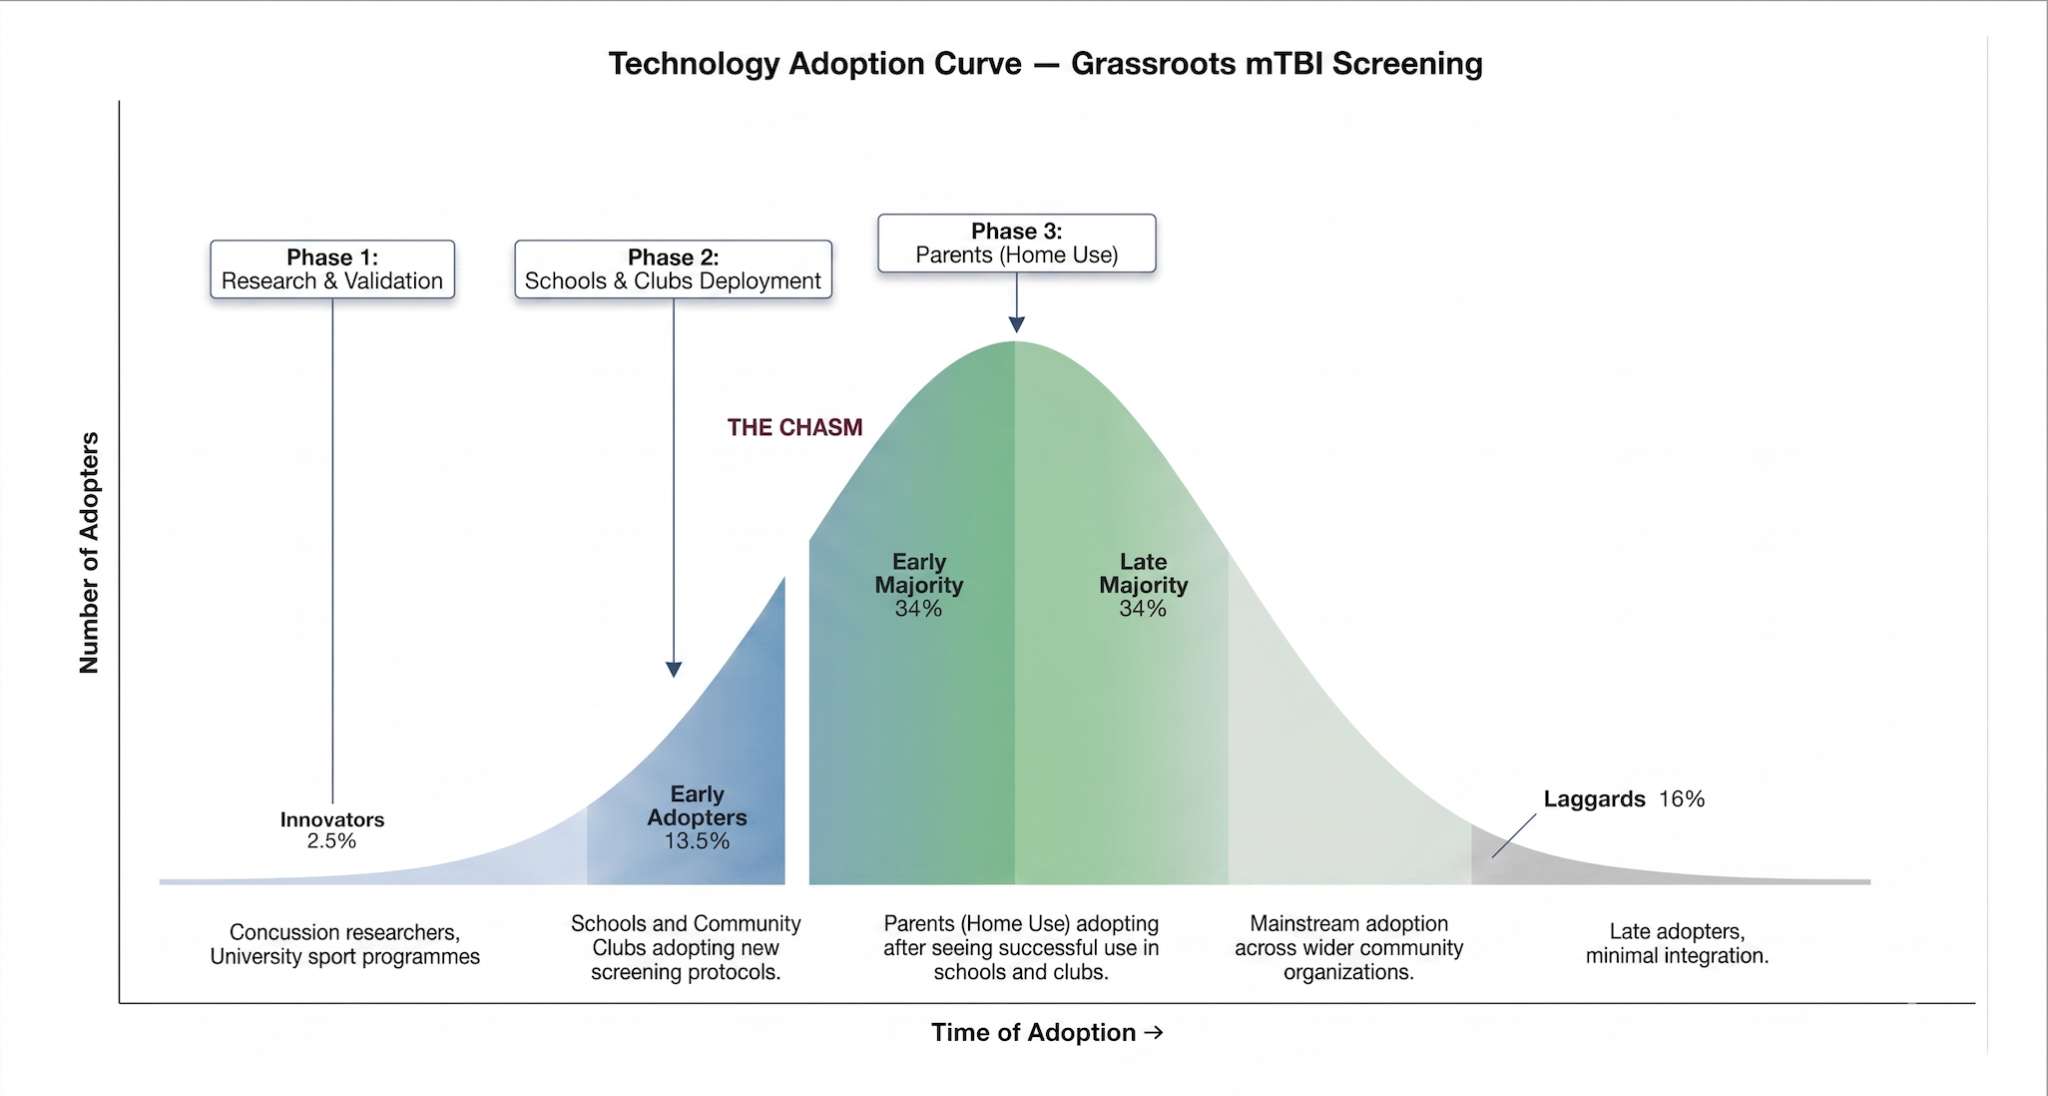
\includegraphics[width=0.85\textwidth]{figures/eem/technology_adoption_curve}
    \caption{Technology adoption curve for grassroots mTBI screening.}
    \label{fig:ent-technology-adoption}
\end{figure}

Using Rogers' diffusion of innovations~\cite{rogers2003diffusion}, Phase 1 consists of innovators which are concussion researchers in this context. They have the frameworks to test unvalidated tools (CUREC) and are motivated by publishing papers and making breakthroughs in emerging fields whilst not requiring a fully functioning product to start testing it. This is advantageous as the product is yet to be regulatory approved here (\Cref{chapter:ent-regulatory}) and under the lean startup build, measure, learn framework~\cite{ries2011lean} this would allow for iteration sequences, converging towards the best product that can be deployed to the market and producing a published validation paper producing strong evidence for acceptance of the stakeholders in Phase 2.

Phase 2 are the early adopters, where schools and youth clubs are targeted. These stakeholders such as the PE teachers, headmasters and coaches will adopt research evidence and institutional endorsement as they see the potential in the product, not because of popularity. This was supported by an interview with a headmaster, a high power, high interest stakeholder in these settings as per the figures below, who said they would ``use it every single time once validated to be safe and useful by experts''. This is typical early adopter behaviour.

The chasm identified by Moore~\cite{moore1991chasm} follows these phases after which we reach Phase 3 with the early majority of the mass market of parents who would want more evidence of a functioning product before using it such as prior use in school, exhibiting early majority behaviour. These last two phases are cumulative; Phase 2 generates institutional validation to assist Phase 3 as well as verifying strategies to expand within the community of schools and clubs which continue through Phase 3 to the mass market of schools, clubs and parents at home.

To justify these claims and sequence of phases to appropriately match the different groups to the characteristics of the phases, these statements were grounded in strong evidence. Appropriate methods covered to support this included user interviews, the ACCORD framework[176], and stakeholder dynamics.

\FloatBarrier
\begin{figure}[!htbp]
    \centering
    \begin{minipage}{0.32\textwidth}
        \centering
        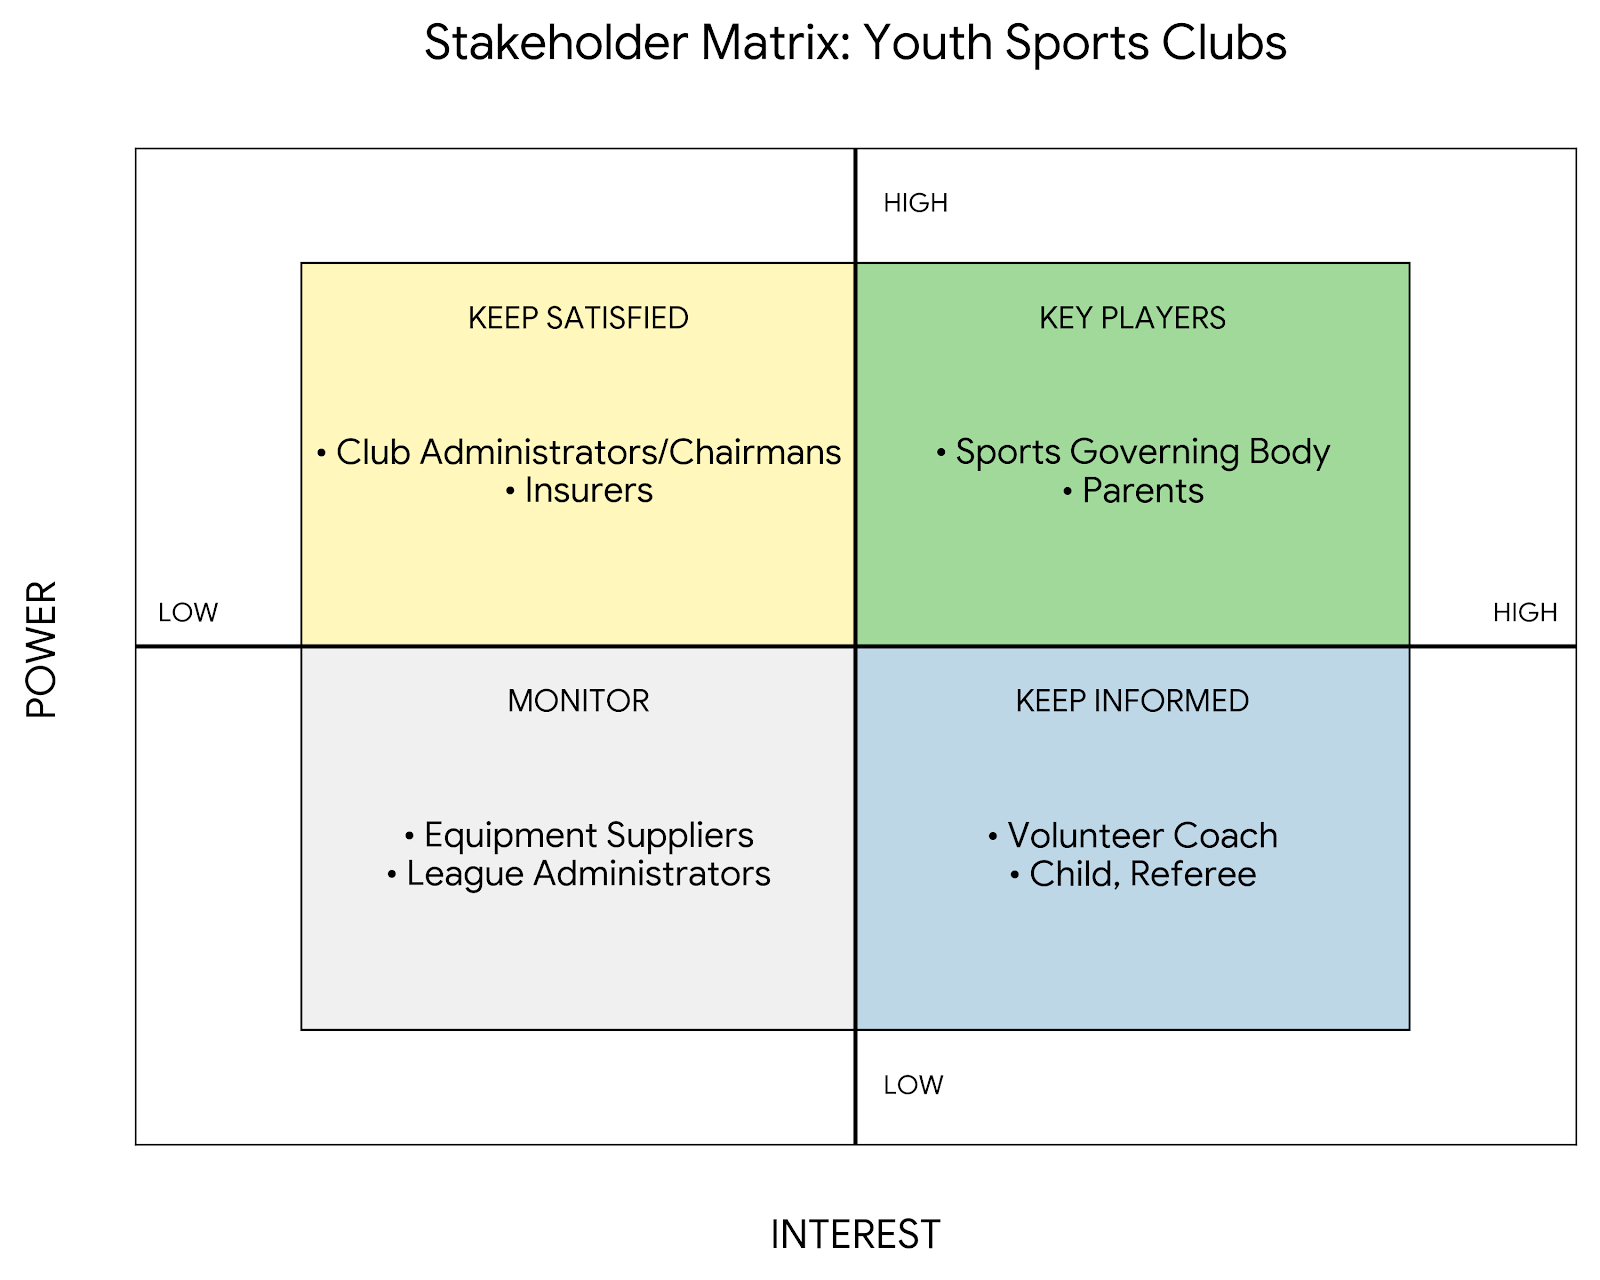
\includegraphics[width=\textwidth]{figures/eem/stakeholder_matrix_youth_sports_clubs}
        \subcaption{Youth sports clubs}
        \label{fig:ent-stakeholder-youth-clubs}
    \end{minipage}\hfill
    \begin{minipage}{0.32\textwidth}
        \centering
        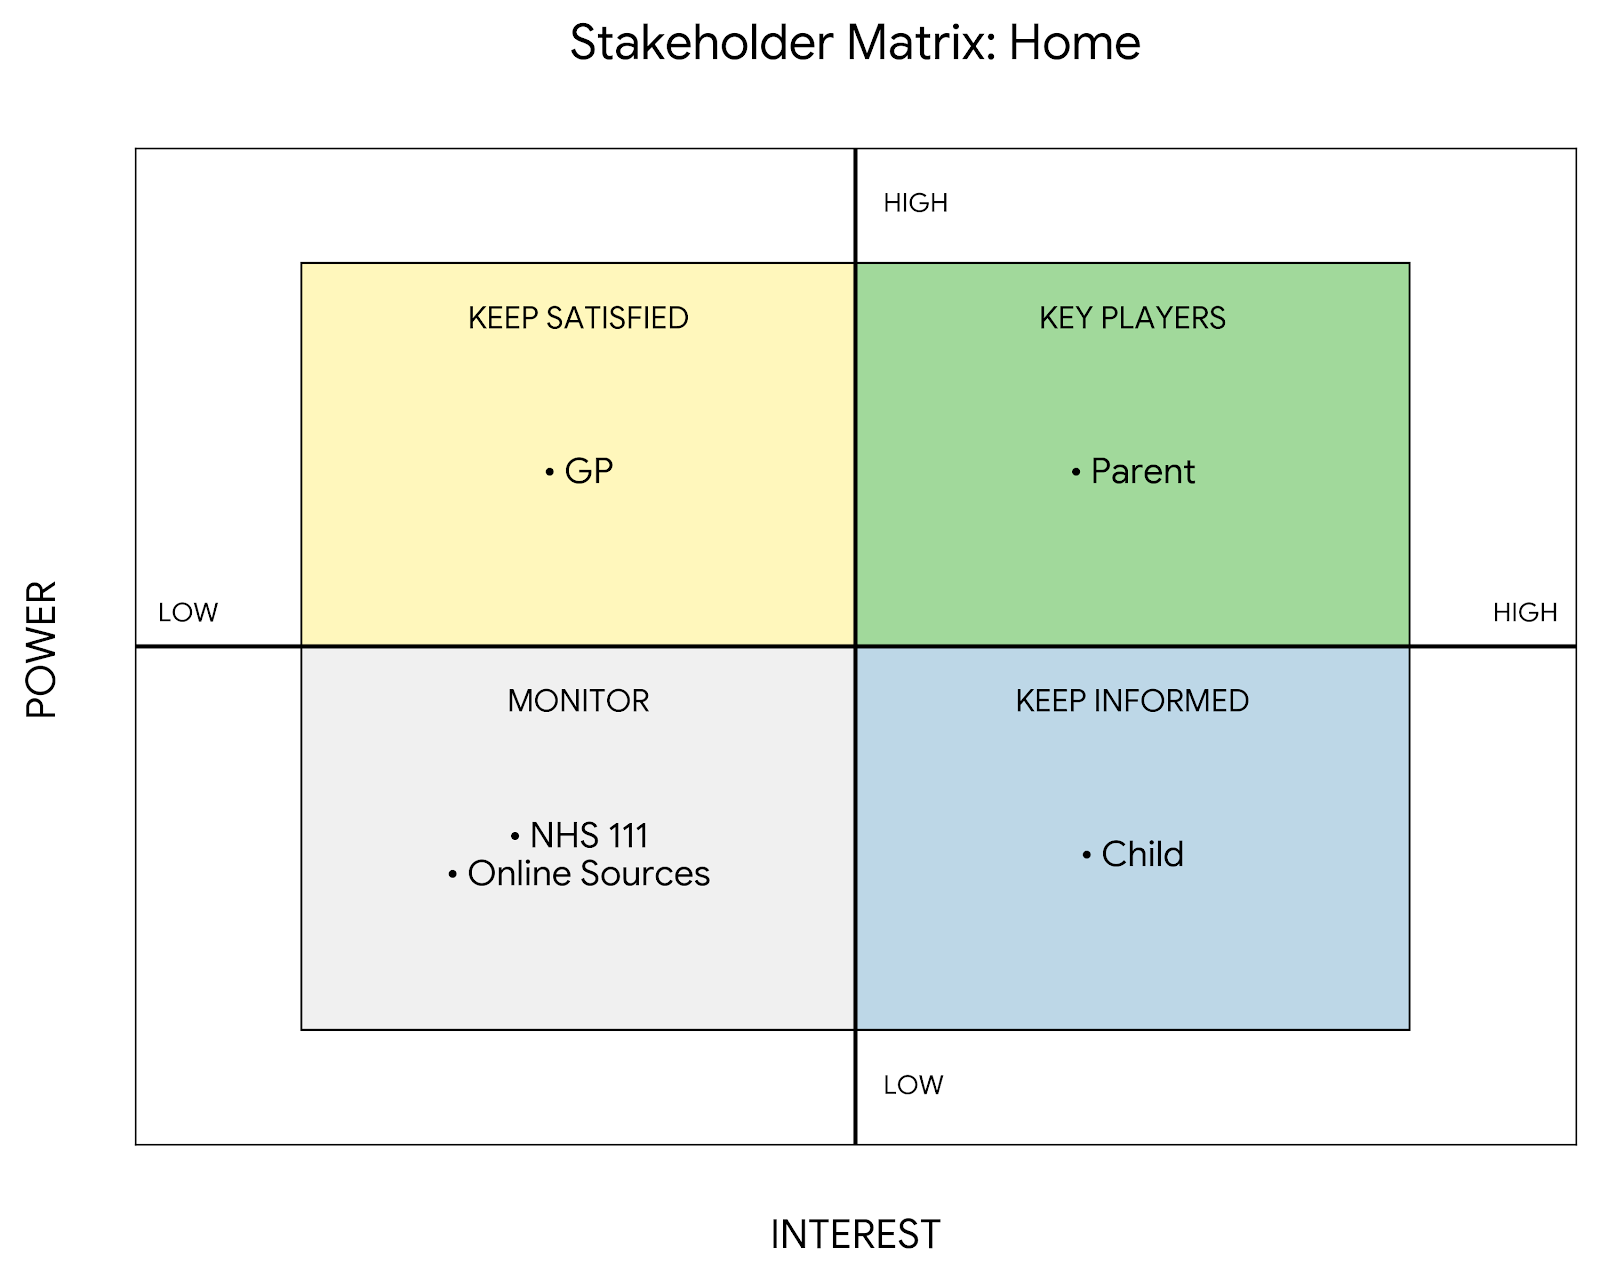
\includegraphics[width=\textwidth]{figures/eem/stakeholder_matrix_home}
        \subcaption{Users at home}
        \label{fig:ent-stakeholder-home}
    \end{minipage}\hfill
    \begin{minipage}{0.32\textwidth}
        \centering
        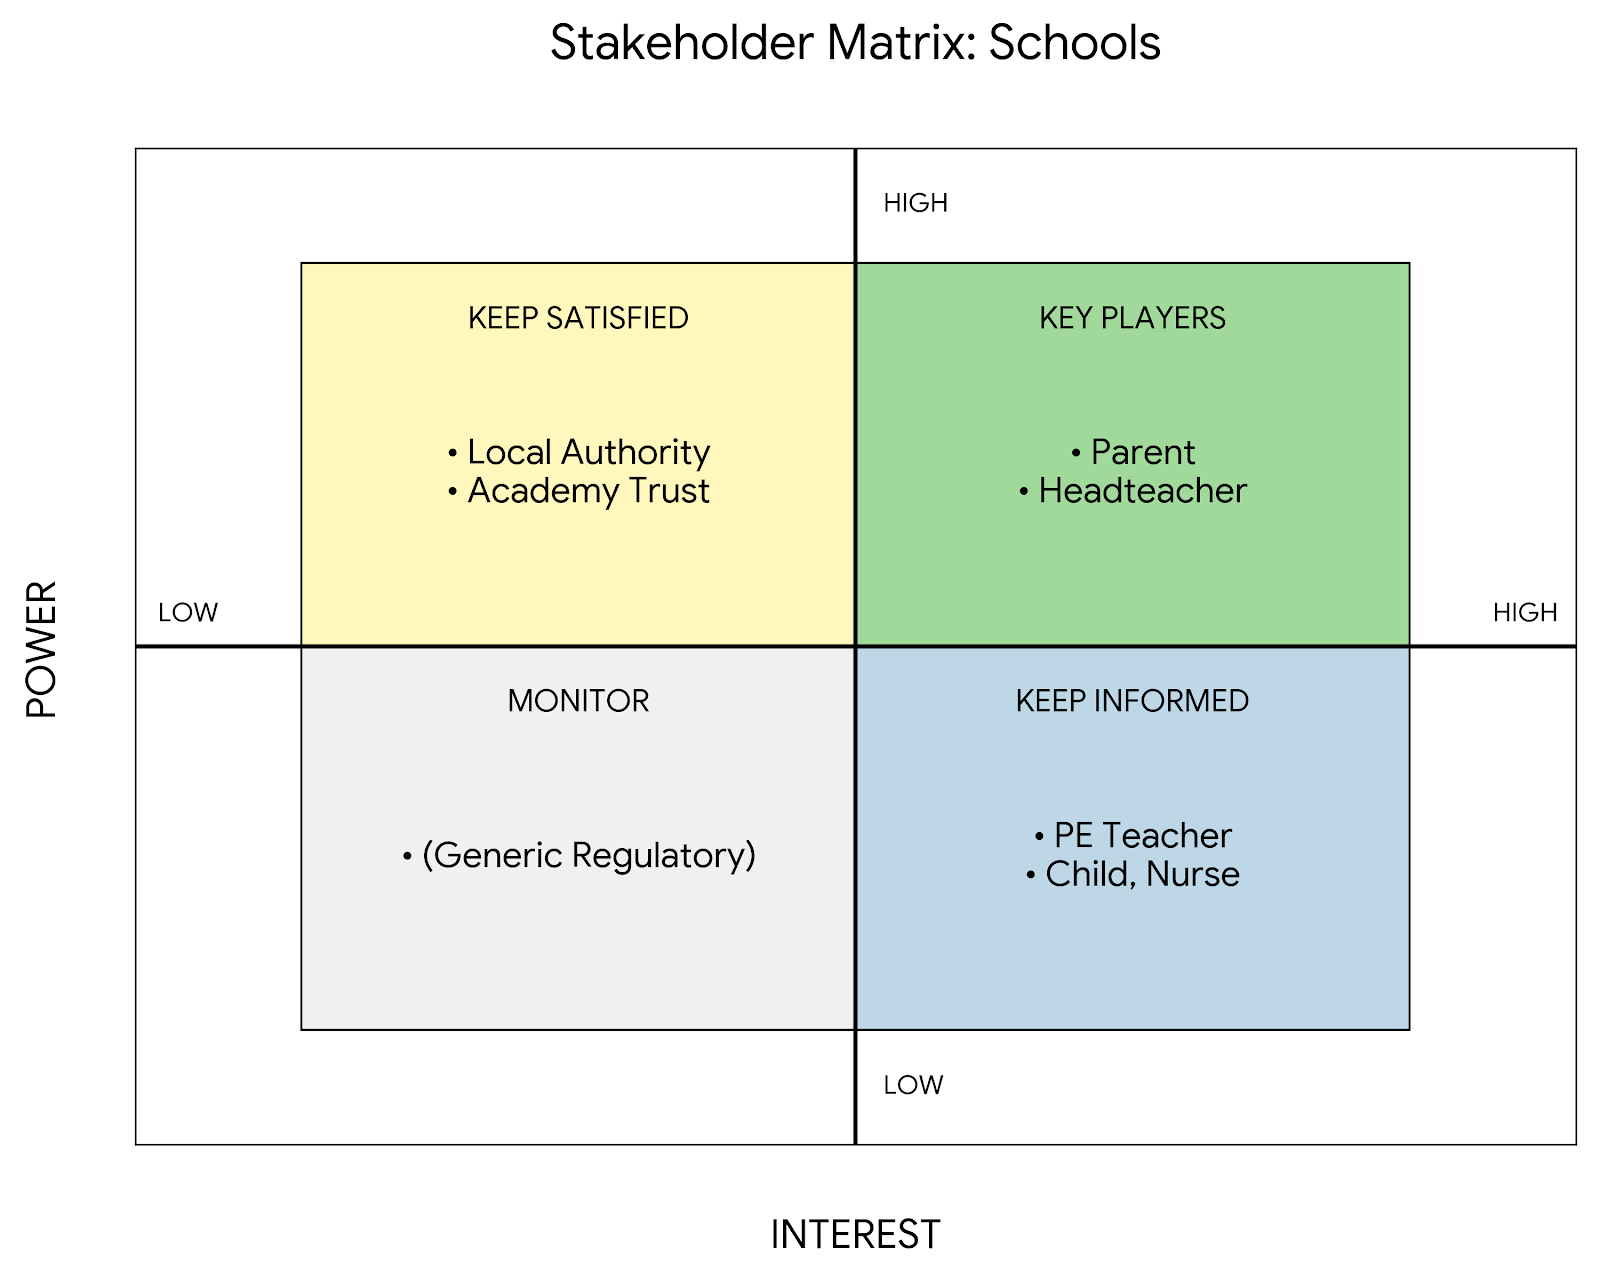
\includegraphics[width=\textwidth]{figures/eem/stakeholder_matrix_schools}
        \subcaption{Users at school}
        \label{fig:ent-stakeholder-schools}
    \end{minipage}
    \caption{Power-interest grids across the three target deployment settings.}
    \label{fig:ent-stakeholder-grids}
\end{figure}
\FloatBarrier

The power interest grids across the different settings of deployment show that parents are persistently high power, high interest stakeholders, driving user interviews to understand what must be in place for them to adopt the product. Statements of parents included ``if 100 schools are using it, I would feel confident'' and ``not something untested'', verifying that there should be sales and validation from schools and clubs before targeting large volume sales to parents.

Additionally, applying the ACCORD framework helps understand how quickly an innovation can be adopted. Analysing this in comparison with and without the prior phase to understand which order is more fruitful relative to each other yielded the following results.

\paragraph{Advantages.} In either case the tool would be better than non-trained coaches and parents by providing an objective measurement that is easy to use. No relative claim could be made here.

\paragraph{Compatibility.} The social compatibility would be relatively larger with Phase 2 than without as using a tool that is used by schools would make the parents feel like they are being a ``good, involved parent'' as verified in a user interview.

\paragraph{Complexity.} For both cases the tool is easy to use, providing low complexity with a simple app interface developed in \Cref{chapter:software}. No relative claim could be made here either.

\paragraph{Observability.} With Phase 2, the observability would be high due to the social proof of the tool being used on pitches and recognisable coaches motivating parents that are watching on the sidelines or hear by word of mouth as per the user interview. Without Phase 2, there would be less evidence for this as they would be beginning at the same time, the amount of observations of the tool's benefit would be lower. This reasoned a relative adoption benefit of having Phase 2 before Phase 3.

\paragraph{Risk.} With Phase 2, the perceived risk would be lower as per the user interview. Without Phase 2 the evidence would not be there to support the parents' worry, pushing favour towards Phase 2.

\paragraph{Divisibility.} With Phase 2, the product would already readily exist among certain schools and clubs at a larger scale than without phase 2, leading to easier trial use, pushing towards relative favour of Phase 2.


\section{Conclusions and Limitations}
\label{sec:ent-roadmap-conclusions}

Through applying the appropriate frameworks, a strong argument was made for pushing forward this adoption sequence. However, the limited number of user interviews, and perhaps a more complicated story of the risk-averse behaviour exhibited by this population, can equally justify selling to parents as soon as there has been regulatory approval. Such an argument could claim if they are risk-averse~\cite{stone2013selfother,dore2014parental}, they would adopt it immediately to help the child.
